\documentclass{article}

% if you need to pass options to natbib, use, e.g.:
% \PassOptionsToPackage{numbers, compress}{natbib}
% before loading nips_2018

% ready for submission
\usepackage[]{nips_2018}

% to compile a preprint version, e.g., for submission to arXiv, add
% add the [preprint] option:
% \usepackage[preprint]{nips_2018}

% to compile a camera-ready version, add the [final] option, e.g.:
% \usepackage[final]{nips_2018}

% to avoid loading the natbib package, add option nonatbib:
% \usepackage[nonatbib]{nips_2018}

\usepackage[utf8]{inputenc} % allow utf-8 input
\usepackage[T1]{fontenc}    % use 8-bit T1 fonts
\usepackage{hyperref}       % hyperlinks
\usepackage{url}            % simple URL typesetting
\usepackage{booktabs}       % professional-quality tables
\usepackage{amsfonts}       % blackboard math symbols
\usepackage{nicefrac}       % compact symbols for 1/2, etc.
\usepackage{microtype}      % microtypography


% The \author macro works with any number of authors. There are
% two
% commands used to separate the names and addresses of multiple
% authors: \And and \AND.
%
% Using \And between authors leaves it to LaTeX to determine where to
% break the lines. Using \AND forces a line break at that point. So,
% if LaTeX puts 3 of 4 authors names on the first line, and the last
% on the second line, try using \AND instead of \And before the third
% author name.
\usepackage{amssymb}
\usepackage{amsmath,amsthm}
\usepackage{float}
\usepackage{url}
\usepackage{setspace}
\usepackage{hyperref}
\usepackage{todonotes}
\usepackage{amsthm} 
\usepackage[ruled,vlined,linesnumbered]{algorithm2e} 
\usepackage{makecell}
\usepackage{upgreek}
\onehalfspacing
\usepackage{pdfpages}
\usepackage{times}
\usepackage{multirow}
\usepackage[toc,page]{appendix}
\usepackage{listings}
\newtheorem{thm}{Theorem}
\newtheorem{lemma}[thm]{Lemma}
\newtheorem{definition}[thm]{Definition}
\newtheorem{observation}[thm]{Observation}
\newtheorem{theorem}[thm]{Theorem}
\newtheorem{claim}[thm]{Claim}
\newtheorem{example}[thm]{Example}
\newtheorem{proposition}[thm]{Proposition}
\usepackage{color,soul}
\usepackage{tikz}
\usetikzlibrary{arrows,shapes.geometric,shapes.arrows}
\usepackage{pgfplots}
\usepackage{multirow}


\DeclareMathOperator{\supp}{support}
\DeclareMathOperator{\support}{support}
\DeclareMathOperator{\Trim}{Trim}
\DeclareMathOperator{\LTrim}{LTrim}
\SetKwFunction{mEqOne}{mEqOne} 
\DeclareMathOperator{\KlmApprox}{KolmogorovApprox}
%\DeclareMathOperator{\OptTrim}{KolmogorovApprox}
\DeclareMathOperator{\OptTrim}{OptTrim}
\title{Kolmogorov Approximation}



\begin{document}
% \nipsfinalcopy is no longer used

\maketitle

\section{Introduction}

Many different approaches to approximation of probability distributions are studied in the literature~\cite{AMCR83,pavlikov2016cvar,PS77}. 
The papers vary in the types random variables involved, how they are represented, and in the criteria used for evaluation of the quality of the approximations. This paper is on approximating discrete distributions represented as explicit probability mass functions with ones that are simpler to store and to manipulate. This is needed, for example, when a discrete distribution is given as a large data-set, obtained, e.g., by sampling, and we want to represent it approximately with a small table.  

The main contribution of this paper is an efficient algorithm for computing the best possible approximation of a given random variable with a random variable whose complexity is not above a prescribed threshold, where the measures of the quality of the approximation and the complexity of the random variable are as specified in the following two paragraphs. 

We measure the quality of an approximation by the distance between the original variable and the approximate one. Specifically, we use the Kolmogorov distance which is one of the most used in statistical practice and literature. Given two random variables $X$ and $X'$ whose cumulative distribution functions (cdfs) are $F_X$ and $F_{X'}$, respectively, the Kolmogorov distance between $X$ and $X'$ is $d_K(X,X')= \sup_t |F_X(t) - F_{X'}(t)|$ (see, e.g.,~\cite{gibbons2011nonparametric}). We say taht $X'$ is a good approximation of $X$ if $d_K(X,X')$ is small.

The complexity of a random variable is measured by the size of its support, the number of values that it can take, $|\support(X)|=|\{x\colon Pr(X=x) \neq 0\}|$. When distributions are maintained as explicit tables, as done in many implementations of statistical software, the size of the support of a variable is proportional to the amount of memory needed to store it and to the complexity of the computations around it. 

In summary, the exact notion of optimality of the approximation targeted in this paper is:
\begin{definition}
	A random variable $X'$ is an optimal $m$-approximation of a random variable $X$ if $|\support(X')| \leq m$ and there is no random variable $X''$ such that $|\support(X'')| \leq m$ and $d_k(X,X'') < d_k(X,X')$.
\end{definition}

The main contribution of the paper is a constructive proof of:
\begin{theorem}
	Given a random variable $X$ and a number $m$, there is an algorithm with memory and time complexity $O(|\support(X)|^2 \cdot m)$  that computes an optimal $m$-approximation of $X$.
\end{theorem}

\section{Related Work}
The problem studied in this paper is related to the theory of Sparse Approximation (aka Sparse Representation) that deals with sparse solutions for systems of linear equations, as follows. 

Given a matrix $D \in \mathbb{R}^{n \times p}$ and a vector $x \in \mathbb{R}^n$, the most studied sparse representation problem is finding the sparsest possible representation $\alpha \in \mathbb{R}^p$ satisfying $x = D\alpha$:
$$
\min_{\alpha \in \mathbb{R}^p} \|\alpha\|_0 \text{ subject to } x = D\alpha.
$$
where $\|\alpha\|_0 = |\{ i : \alpha_i \neq 0, \, i=1,\ldots,p \}|$ is the $\ell_0$ pseudo-norm, counting the number of non-zero coordinates of $\alpha$. This problem is known to be NP-Hard with a reduction to NP-complete subset selection problems.

In these terms, using also the $\ell_\infty$ norm that represents the maximal coordinate and the $\ell_1$ norm that represents the sum of the coordinates, our problem can be phrased as:
$$
\min_{\alpha \in \mathbb{R}^p_{\geq 0}}\|x - D\alpha\|_{\infty} \text{ subject to }  \|\alpha\|_0 = m \text{ and } \|\alpha\|_1=1.
$$
where $D$ is the all-ones triangular matrix (the entry at row $i$ and column $j$ is one if $i\leq j$ and zero otherwise), $x$ is related to $X$ such that the $i$th coordinate of $x$ is $F_X(x_i)$ where $\support(X)=\{x_1 < x_2 < \cdots < x_n\}$ and $\alpha$ is related to $X'$ such that the $i$th coordinate of $\alpha$ is $f_{X'}(x'_i)$ where $\support(X')=\{x'_1 < x'_2 < \cdots < x'_m\}$. The functions $F_X$ and $f_{X'}$ represent, receptively, the cumulative distribution function of $X$ and the mass distribution function of $X'$. This, of course, means that the coordinates of $x$ are assumed to be positive and monotonically increasing and that the last coordinate of $x$ must be one. We demonstrate an application for this specific sparse representation problem and show that it can be solve in $O(n^2m)$ time and memory.




\section{An Algorithm for Optimal Approximation}


\begin{itemize}
	\item We now start our story: Given $X$ and $m$ how can we find $X'$?
	\item We first show that it is enough to limit our search to $X'$s such that $\support(X') \subseteq \support(X)$.
\end{itemize}

\begin{lemma}
	For any discrete random variable $X$ and any $m \in \mathbb{N}$, there is an $m$-optimal-approximation $X'$ of $X$ such that $\support(X') \subseteq \support(X)$.
\end{lemma}
\begin{proof}
Assume there is a random variable $X''$ with support size $m$ such that $d_K(X,X'')$ is minimal but $\support(X'')\nsubseteq\support(X)$.
We will show how to transform $X''$ support such that it will be contained in $\support(X)$. Let $v'$ be the first $v'\in\support(X'')$ and $v' \not\in\support(X)$. Let $v=\max\{i: i<v' \wedge i\in\support(X)\}$. Every $v'$ we will replace with $v$ and name the new random variable $X'$, we will show that $d_K(X,X'') = d_K(X,X')$. First, note that:
$F_{X''}(v')=F_{X'}(v)$, $F_{X}(v')=F_{X}(v)$.
Second,  $F_{X'}(v')-F_{X}(v') = F_{X'}(v)-F_{X}(v)$. Therefore, $d_K(X,X'') = d_K(X,X')$ and $X'$ is also an optimal approximation of $X$.
\end{proof}

\begin{observation}\label{obs:ab}
	$max\{|a|,|b|\} \geq |a-b|/2$
\end{observation}
%\begin{proof}
%$$ \frac{|a-b|}{2}	\leq \frac{|a|+|b|}{2} \leq  \max\{|a|,|b|\}.$$
%\end{proof}

\begin{itemize}
	\item The next lemma states a lower bound on the distance $d_K(X,X')$ when a range of elements is excluded from the support of $X'$.
\end{itemize}


\begin{lemma}\label{lem:geq}
	For $x_1, x_2 \in \support(X) \cup \{-\infty,\infty\}$ such that $x_1 < x_2$, if $P(x_1 < X' < x_2)=0$  then 
	$d_k(X,X') \geq P(x_1 < X < x_2)/2$.
\end{lemma}
\begin{proof}
	Let $\hat x=\max \{x \in \support(X) \cap\{ -\infty, \infty\}  \colon x < x_2 \}$. By definition, $d_k(X,X') \geq \max \{|F_X(x_1) - F_{X'}(x_1)|, |F_X(\hat x) - F_{X'}(\hat x)| \}$. From Observation~\ref{obs:ab}, $d_k(X,X') \geq 1/2|F_X(x_1) - F_X(\hat x) + F_{X'}(\hat x) - F_{X'}(x_1)|$. Since it is given that $F_{X'}(\hat x) - F_{X'}(x_1) = P(x_1 < X' < x_2)=0$, $d_k(X,X') \geq 1/2|F_X(x_1) - F_X(\hat x) | =  P(x_1 < X \leq \hat x)/2 = P(x_1 < X < x_2)/2$.
\end{proof}


\begin{itemize}
	\item The next lemma strengthen the lower bound.
\end{itemize}


\begin{lemma}\label{lem:geq2}
	For $x_1, x_2 \in \support(X) \cup \{-\infty,\infty\}$ such that $x_1=-\infty$ or  $x_2=\infty$, if $P(x_1 < X' < x_2)=0$  then 
	$d_k(X,X') \geq P(x_1 < X < x_2)$.
\end{lemma}
\begin{proof}
	Let $\hat x=\max \{x \in \support(X) \cap\{ -\infty, \infty\}  \colon x < x_2 \}$. By definition $d_k(X,X') \geq \max \{|F_X(x_1) - F_{X'}(x_1)|, |F_X(\hat x) - F_{X'}(\hat x)| \}$. If $x_1=-\infty$ then $d_k(X,X') \geq \{|F_X(\hat x) - F_{X'}(\hat x)| \}$ since $F_X(-\infty) = F_{X'}(-\infty) = 0$. Furthermore, $F_{X'}(\hat x) = P(x_1 < X' < x_2)=0$. Therefore $d_k(X,X') \geq F_X(\hat x) = P(x_1 < X \leq \hat x) = P(x_1 < X < x_2)$. 
	If $x_2=\infty$ then $d_k(X,X') \geq \{|F_X(x_1) - F_{X'}(x_1)| \}$ since $F_X(\hat{x}) = F_{X'}(\hat{x}) = F_X(\infty) = F_{X'}(\infty) = 1$. Furthermore, $F_{X'}(x_1) = 1$ since it is given that $P(x_1 < X' < x_2)=0$. Therefore we get that $d_k(X,X') \geq |F_X(x_1)-1| = |1-F_X(\hat x)-| = P(x_1 < X \leq \hat x) = P(x_1 < X < x_2)$.
\end{proof}


\begin{definition}\label{def:weight} For $x_1,x_2 \in \support(X) \cup \{-\infty,\infty\}$ let
	\[
	w(x_1,x_2)=
	\begin{cases}
		P(x_1 < X < x_2) & \text{if $x_1=-\infty$ or $x_2 = \infty$;} \\
		P(x_1 < X < x_2)/2 & \text{otherwise.} \\	
	\end{cases}
	\]
\end{definition} 


\begin{definition}\label{def:error} For $S=\{x_1<\dots<x_m\} \subseteq \support(X)$, $x_0=-\infty$, and $x_{m+1}=\infty$, let
	\[
	\varepsilon(X,S) = \max\limits_{i=0,\dots,m} w(x_{i}, x_{i+1}).
	\]
\end{definition} 

\begin{itemize}
	\item From here on, until the end of the section, $S$ is fixed.
\end{itemize}



\begin{proposition}
	There is no $X'$ such that $\support(X')=S$ and $d_k(X,X') < \varepsilon(X,S)$.
\end{proposition}
\begin{proof}
	Let $i$ be the index that maximizes $w(x_{i}, x_{i+1})$. If $0<i<n-1$ then $d_k(X,X') \geq w(x_{i}, x_{i+1})$ by Lemma~\ref{lem:geq}. If $i=0$ or $i=n+1$ the same follows from Lemma~\ref{lem:geq2}.
\end{proof}

\begin{definition}\label{def:construction}
Let $X'$ to by $f_{X'}(x_{i}) = w(x_{i-1},x_i) + w(x_i,x_{i+1}) + f_{X}(x_i)$ for $i=1,\dots,m$ and $f_{X'}(x)=0$ for $x \notin S$.
\end{definition}

\begin{lemma}
	For $i>1$, if $F_{X'}(x_{i})-F_{X}(x_{i}) = w(x_{i}, x_{i+1})$ then $F_{X'}(x_{i+1})-F_{X}(x_{i+1}) = w(x_{i+1}, x_{i+2})$.
\end{lemma}
\begin{proof}
	\begin{align}
	&F_{X'}(x_{i+1})-F_{X}(x_{i+1}) = \\ \nonumber
	& = f_{X'}(x_{i+1}) - f_{X}(x_{i+1}) - P(X<x_{i+1}) + P(X'<x_{i+1})  \\ \nonumber
	& = f_{X'}(x_{i+1}) - f_{X}(x_{i+1}) - F_X(x_{i}) - P(x_{i}< X < x_{i+1}) + F_{X'}(x_{i}) \\ 
	\label{eq:weight}
	& = f_{X'}(x_{i+1}) - f_{X}(x_{i+1}) - F_X(x_{i}) - 2w(x_{i},x_{i+1}) + F_{X'}(x_{i})  \\ \label{eq:indHip}
	& = f_{X'}(x_{i+1}) - f_{X}(x_{i+1}) - 2w(x_{i},x_{i+1}) +w(x_{i}, x_{i+1})  \\ \label{eq:construction}
	& = w(x_{i},x_{i+1}) +w(x_{i+1},x_{i+2}) - 2w(x_{i},x_{i+1}) +w(x_{i}, x_{i+1}) \\ \nonumber
	& = w(x_{i+1},x_{i+2}) \nonumber
	\end{align}
	
	By Definition~\ref{def:weight} the probability $P(x_{i-1}< X < x_i) = 2w(x_{i-1},x_{i})$ as in Equation~\eqref{eq:weight}. Equation~\eqref{eq:indHip} is deduced by the induction hypothesis and Equation~\eqref{eq:construction} where
	$f_{X'}(x_i) - f_{X}(x_i) = w(x_{i-1},x_i) + w(x_i,x_{i+1})$ is true by construction, see Definition\ref{def:construction}.
\end{proof}

%\begin{lemma}
%	For $i>1$, if $F_{X'}(x_{i-1})-F_{X}(x_{i-1}) = w(x_{i-1}, x_{i})$ then $F_{X'}(x_{i})-F_{X}(x_i) = w(x_i, x_{i+1})$.
%\end{lemma}
%\begin{proof}
%	% TODO switch tdirections to fit the statement of the lemma
%	% TODO \eqref,  aligment
%	\begin{align}
%	&F_X(x_i)-F_{X'}(x_i) = \\
%	&f_{X}(x_i) - f_{X'}(x_i) + P(X<x_i) - P(X'<x_i)  = \\ \nonumber
%	&f_{X}(x_i) - f_{X'}(x_i) + F_X(x_{i-1}) + P(x_{i-1}< X < x_i)-F_{X'}(x_{i-1}) = \\
%	&f_{X}(x_i) - f_{X'}(x_i) + F_X(x_{i-1}) + 2w(x_{i-1},x_{i})-F_{X'}(x_{i-1}) =^* \\
%	&f_{X}(x_i) - f_{X'}(x_i) + 2w(x_{i-1},x_{i}) -w(x_{i-1}, x_{i}) = \\
%	& -w(x_{i-1},x_i) - w(x_i,x_{i+1}) + 2w(x_{i-1},x_{i}) -w(x_{i-1}, x_{i}) =\\ 
%	&- w(x_i,x_{i+1})
%	\end{align}
%	$*$ by induction hypothesis.
%	The probability $P(x_{i-1}< X < x_i) = 2w(x_{i-1},x_{i})$ by Definition~\ref{def:weight}, and
%	$f_{X'}(x_i) - f_{X}(x_i) = w(x_{i-1},x_i) + w(x_i,x_{i+1})$ by construction.
%\end{proof}

\begin{lemma}
	Base case: $i = 1, F_{X'}(x_{1})-F_{X}(x_{1}) = w(x_{1}, x_{2})$.
\end{lemma}
\begin{proof}
	\begin{align*}
	F_{X'}(x_{1})-F_{X}(x_{1}) &= \\
	& = f_{X'}(x_{1}) - f_{X}(x_{1}) - w(x_0, x_1)  \\
	& = w(x_{0},x_1) + w(x_1,x_{2}) - w(x_0, x_1)  \\
	& = w(x_1,x_{2})
	\end{align*}
\end{proof}




\begin{proposition}
	There exists $X'$ such that $\support(X')=S$ and $d_k(X,X') = \varepsilon(X,S)$.
\end{proposition}
%\begin{proof}
%	Define $X'$ to by $f_{X'}(x_i) = w(x_{i-1},x_i) + w(x_i,x_{i+1}) + f_{X}(x_i)$ for $i=1,\dots,m$ and $f_{X'}(x)=0$ for $x \notin S$.
%	We need to show that $F_X(x_i)-F_{X'}(x_i) = -w(x_i, x_{i+1})$. Assume this is true for every $j<i$, the induction hypothesis hereby: $F_X(x_{i-1})-F_{X'}(x_{i-1}) = -w(x_{i-1}, x_{i})$.
%	\begin{align*}
%		&F_X(x_i)-F_{X'}(x_i) = \\
%		&f_{X}(x_i) - f_{X'}(x_i) + P(X<x_i) - P(X'<x_i)  = \\
%		&f_{X}(x_i) - f_{X'}(x_i) + F_X(x_{i-1}) + P(x_{i-1}< X < x_i)-F_{X'}(x_{i-1}) = \\
%		&f_{X}(x_i) - f_{X'}(x_i) + F_X(x_{i-1}) + 2w(x_{i-1},x_{i})-F_{X'}(x_{i-1}) =^* \\
%		&f_{X}(x_i) - f_{X'}(x_i) + 2w(x_{i-1},x_{i}) -w(x_{i-1}, x_{i}) = \\
%		& -w(x_{i-1},x_i) - w(x_i,x_{i+1}) + 2w(x_{i-1},x_{i}) -w(x_{i-1}, x_{i}) =\\ 
%		&- w(x_i,x_{i+1})
%	\end{align*}
%	$*$ by induction hypothesis.
%	The probability $P(x_{i-1}< X < x_i) = 2w(x_{i-1},x_{i})$ by definition~\ref{def:weight}, and
%	$f_{X'}(x_i) - f_{X}(x_i) = w(x_{i-1},x_i) + w(x_i,x_{i+1})$ by construction.
%	
%\end{proof}



%\begin{proposition}
%	For any random variable $X$ and an ordered set $S=\{x_1<\dots<x_m\} \subset \support(X)$ there is no random variable $X'$ such that $\support(X')=S$ and $d_k(X,X') < \max\limits_{i=0,\dots,m} w(x_{i}, x_{i+1})$ where, to simplify notations, we assume that $x_0=-\infty$ and $x_{m+1}=\infty$.
%\end{proposition}
%
%\begin{proof}
%	Let $i$ be the index that maximizes $w(x_{i}, x_{i+1})$. If $0<i<n-1$ then $d_k(X,X') \geq w(x_{i}, x_{i+1})$ by Lemma~\ref{lem:geq}. If $i=0$ or $i=n+1$ the same follows from Lemma~\ref{lem:geq2}.
%\end{proof}
%
%\begin{itemize}
%	\item The next lemma shows that there is a n not better approximation. 
%\end{itemize}
%
%
%
%\begin{proposition}
%	For any random variable $X$ and an ordered set $S=\{x_1<\dots<x_m\} \subset \support(X)$ there is a random variable $X'$ such that $\support(X')=S$ and $d_k(X,X') = \max\limits_{i=0,\dots,m} w(x_{i}, x_{i+1})$ where, to simplify notations, we assume that $x_0=-\infty$ and $x_{m+1}=\infty$.
%\end{proposition}
%\begin{proof}
%Define $X'$ to by $f_{X'}(x_i) = w(x_{i-1},x_i) + w(x_i,x_{i+1}) + f_{X}(x_i)$ for $i=1,\dots,m$ and $f_{X'}(x)=0$ for $x \notin S$.
%\end{proof}

Chakravarty, Orlin, and Rothblum~\cite{chakravarty1982partitioning} proposed a polynomial-time method that, given certain objective functions (additive), finds an optimal consecutive partition. Their method involves the construction of a graph such that the (consecutive) set partitioning problem is reduced to the problem of finding the shortest path in that graph.

The $\KlmApprox$ algorithm (Algorithm~\ref{alg:optapprox}) starts by constructing a directed weighted graph $G$ similar to the method of Chakravarty, Orlin, and Rothblum~\cite{chakravarty1982partitioning}. The nodes $V$ consist of the support of $X$ together with an extra two nodes, $-\infty$ and $\infty$ for technical reasons, whereas the edges $E$ connect every pair of nodes in one direction (lines 1-2). The weight $w$ of each edge $e=(i,j)\in E$ is determined by one of two cases as in Definition~\ref{def:weight}. The first is where $i$ or $j$ are the source or target nodes respectively. In this case the weight is the probability of $X$ to get a value between $i$ and $j$, non inclusive, i.e., $w(e)=Pr(i<X<j)$ (lines 4-5). The second case is where $i$ or $j$ are not a source or target nodes, here the weight is the probability of $X$ to get a value between $i$ and $j$, non inclusive, divided by two i.e., $w(e)=Pr(i<X<j)/2$ (lines 6-7). The values taken are non inclusive, since we are interested only in the error value.
The source node of the shortest path problem at hand corresponds to the $-\infty$ node added to $G$ in the construction phase, and the target node is the extra node $\infty$.
The set of all solution paths in $G$, i.e., those starting at $-\infty$ and ending in $\infty$ with at most $m$ edges, is called $paths(G, -\infty, \infty)$. The goal is to find the path $l$ in $paths(G, -\infty, \infty)$ with the lightest bottleneck (lines 8-9). This can be achieved by using the $Bellman-Ford$ algorithm with two tweaks. The first is to iterate the graph $G$ in order to find only paths with length of at most $m$ edges. The second is to find the lightest bottleneck as opposed to the traditional objective of finding the shortest path. This is performed by modifying the manner of ``relaxation'' to $bottleneck(x) = min[max(bottleneck(v),w(e))]$, done also in~\cite{shufan2011two}. Consequently, we find the lightest maximal edge in a path of length $\leq m$, which represents the minimal error, $\varepsilon(X,S)$, defined in Definition~\ref{def:error} where the nodes in path $l$ represent the elements in set $S$. The approximated random variable $X'$ is then derived from the resulting path $l$ (lines 10-17). Every node $n \in l$ represent a value in the new calculated random variable $X'$, we than iterate the path $l$ to fine the probability of the event $f_{X'}(n)$ as described in Definition~\ref{def:construction}. For every edge $(i,j)\in l$ we determine: if $(i,j)$ is the first edge in the path $ l$ (i.e.  $i==-\infty$), then node $j$ gets the full weight $w(i,j)$ and it's own weight in $X$ such that $f_{X'}(j) = f_{X}(j) +  w(i,j)$ (lines 11-12). If $(i,j)$ in not the first nor the last edge in path $l$ then we divide it's weight between nodes $i$ and $j$ in addition to their own original weight in $X$ and the probability that already accumulated (lines 16-17). If $(i,j)$ is the last edge in the path $ l$ (i.e.  $i==\infty$) then node $i$ gets the full weight $w(i,j)$ in addition to what was already accumulated such that $f_{X'}(j) = f_{X'}(j) +  w(i,j)$ (lines 13-14).



\begin{algorithm}\label{alg:optapprox}
	\DontPrintSemicolon
	\SetKwFunction{Convolv}{Conv}
	\SetKwFunction{getPartition}{getPartition}
	\SetKwFunction{bellmanFordMinMaxM}{bellmanFordMinMaxM}
	$S = \support(X)\cup \{\infty,-\infty\}$\;
	$G=(V,E)=(S, \{ e=(x,y) \in S^2 \colon  x<y \})$  \;
	$ l = \operatorname{argmin}\limits_{l \in paths(G,-\infty,\infty),|l|\leq m}  \max \{ w(e)\colon e \in l  \}$  \;
	\For{$0<i<m+1$ }{
		$f_{X'}(x_{i}) = w(x_{i-1},x_i) + w(x_i,x_{i+1}) + f_{X}(x_i)$
	}	
	\Return $X'$\;
	
	\caption{$\KlmApprox (X, m)$}  
	\label{alg:sequence}
\end{algorithm}


\begin{algorithm}\label{alg:optapprox}
	\DontPrintSemicolon
	\SetKwFunction{Convolv}{Conv}
	\SetKwFunction{getPartition}{getPartition}
	\SetKwFunction{bellmanFordMinMaxM}{bellmanFordMinMaxM}
	$S = \support(X)\cup \{\infty,-\infty\}$\;
	$G=(V,E)=(S, \{e= (x,y) \in S^2 \colon  x<y \})$ \;
	
	\ForEach{$e=(x,y) \in  E $ }{
		\If {$i=\infty \text{ OR } j=-\infty$}{
			$w(e) = Pr(i<X<j)$
		}
		\Else{$w(e) = Pr(i<X<j)/2$}
	}
	
	/* The following can be obtained, e.g., using the Bellman-Ford algorithm */\;
	$l^*= \operatorname{argmin}\limits_{l \in paths(G, -\infty, \infty,|l|\leq m}  \max \{ w(e)\colon e \in l  \}$ \;
	
	\ForEach{$e=(i,j) \in  l^* $ }{
		\If {$i=-\infty$}{
			$f_{X'}(j) = f_{X}(j) + Pr(i\leq X<j)$
		}
		\ElseIf{$j==\infty$}{
			$f_{X'}(i) = f_{X'}(i) + Pr(i\leq X<j)$
		}
		\Else{
			$f_{X'}(i) = f_{X'}(i) + Pr(i\leq X<j)/2$\;
			$f_{X'}(j) = f_{X}(j) + Pr(i\leq X<j)/2$\;
		}
		
	}	
	\Return $X'$\;
	
	\caption{$\KlmApprox (X, m)$}  
	\label{alg:sequence}
\end{algorithm}

\begin{theorem}\label{the:algo}
	$\KlmApprox(X,m) = X' $ where $X'$ is an $m$-optimal-approximation.
\end{theorem}


\begin{theorem}\label{the:complexity}
	The $\KlmApprox(X,m)$ algorithm runs in time $O(mn^2)$, using $O(n^2)$ memory where $n=|\support(X)|$.
\end{theorem}

\begin{proof}
	Constructing the graph $G$ takes $O(n^2)$. The number of edges is $O(E)\approx O(n^2)$ and for every edge the weight is at most the sum of all probabilities between the source node $-\infty$ and the target node $\infty$, which can be done efficiently by aggregating the weights of already calculated edges. 
	The construction is also the only stage that requires memory allocation, specifically $O(E+V)=O(n^2)$.
	Finding the shortest path takes $O(m(E+V))\approx O(mn^2)$. Since $G$ is DAG (directed acyclic graph) finding shortest path takes $O(E+V)$. We only need to find paths of length $\leq m$, which takes $O(m(E+V))$.
	Deriving the new random variable $X'$ from the computed path $l$ takes $O(mn)$. For every node in $l$ (at most $m$ nodes), calculating the probability $P(s<X<\infty)$ takes at most $n$. 
	To conclude, the worst case run-time complexity is $O(n^2+mn^2+mn)=O(mn^2)$ and memory complexity is $O(E+V)=O(n^2)$.
\end{proof}

%\begin{example}\textbf{Why one sided Kolmogorov approximation in not sufficient in this case?}
%	Consider the following random variable $X$: 
%	$$
%	f_{X}(t) = \begin{cases}
%	1/3           & \text{if $t=1$ or $t=2$} ;  \\ 
%	1/6           & \text{if $t=3$ or $t=4$};  \\  
%	0             & \text{otherwise.}
%	\end{cases}
%	$$
%	
%	There are various partitioned random variables of size $m=2$ which provide some approximation in regards to Kolmogorov distance, some are presented as follows:
%	$$
%	f_{X'_1}(t) = \begin{cases}
%	2/3           & \text{if } t=1;  \\ 
%	1/3           & \text{if } t=3;  \\  
%	0             & \text{otherwise.}
%	\end{cases}
%	$$
%	In this case $d_K(X, X'_1) = 1/3$.
%	
%	$$
%	f_{X'_2}(t) = \begin{cases}
%	1/3           & \text{if } t=1;  \\ 
%	2/3           & \text{if } t=2;  \\  
%	0             & \text{otherwise.}
%	\end{cases}
%	$$
%	In this case $d_K(X, X'_2) = 1/3$.
%	
%	$$
%	f_{X'_3}(t) = \begin{cases}
%	2/3           & \text{if } t=2;  \\ 
%	1/3           & \text{if } t=3;  \\  
%	0             & \text{otherwise.}
%	\end{cases}
%	$$
%	In this case $d_K(X, X'_3) = 1/3$.
%	
%	However, none of the above random variables provides an optimal approximation. Here is an optimal approximation which can not be achieved by a regular partitioned random variable:
%	
%	$$ 	f_{X''}(t) = \begin{cases}
%	1/2           & \text{if } t=1;  \\ 
%	1/2           & \text{if } t=3;  \\  
%	0             & \text{otherwise.}
%	\end{cases}
%	$$
%	In this case $d_K(X, X'') = 1/6$.
%\end{example}

\section{Experiments and Results}
In the first experiment we focus on the problem of task trees with deadlines, and consider three types of task trees.
The first type includes logistic problems of transporting packages by trucks and airplanes (from IPC2 http://ipc.icaps-conference.org/). Hierarchical plans of those logistic problems were generated by the JSHOP2 planner \cite{nau2003shop2} (see example problem, Figure~\ref{fig:logistics}). 
The second type consists of task trees used as execution plans for the ROBIL team entry in the DARPA robotics challenge (DRC simulation phase), and the third type is of linear plans (sequential task trees).
The primitive tasks in all the trees are modeled as discrete random variables with support of size $M$ obtained by discretization of uniform distributions over various intervals. The number of tasks in a tree is denoted by $N$. 
\begin{figure}[htb]
	\centering  
	\tiny
	\tikzset{
		node distance=.8cm,
		basic/.style  = {draw
			, text width=2.1cm
			, font=\sffamily \scriptsize, rectangle
		},
		root/.style   = {basic, text width=2.5cm, trapezium,trapezium left angle=70,trapezium right angle=-70, thin, align=center},
		level 2/.style = {basic, ,single arrow, thin, align=left
		},
		level 3/.style = {basic, thin, align=left
		},
	}
	
	\scalebox{0.8}{
		\begin{tikzpicture}
		[
		level 1/.style={
			sibling distance=40mm
		},
		edge from parent/.style={->,draw},
		>=latex]
		
		% root of the the initial tree, level 1
		\node[root] {(transport-two p1 p2)}
		% The first level, as children of the initial tree
		child {node[level 2 ] (c1) {(transport p1)}}
		child {node[level 2] (c2) {(transport p2)}};
		
		% The second level, relatively positioned nodes
		\begin{scope}[every node/.style={level 3}]
		
		\node [single arrow, below of = c1, xshift=20pt] (c11) {(dispatch t1 l1)};
		\node [below of = c11, xshift=20pt] (c111) {(reserve t1)};
		\node [below of = c111] (c112) {(move t1 home l1
			)};
		
		\node [below of = c112, xshift=-20pt] (c12) {(load t1 p1)};
		\node [ below of = c12,] (c13) {(move t1 l1 l3)};
		\node [single arrow,below of = c13,] (c14) {(return t1 l1
			)};
		\node [below of = c14, xshift=20pt] (c141) {(free t1)};
		\node [below of = c141] (c142) {(move t1 l3 home
			)};
		
		
		\node [single arrow,below of = c2, xshift=20pt] (c21) {(dispatch t2 l2)};
		\node [below of = c21, xshift=20pt] (c211) {(reserve t2)};
		\node [below of = c211] (c212) {(move t2 home l2)};
		
		\node [below of = c212, xshift=-20pt] (c22) {(load t2 p2)};
		\node [below of = c22] (c23) {(move t2 l2 l3)};
		\node [single arrow,below of = c23] (c24) {(return t2 l2)};
		\node [below of = c24, xshift=20pt] (c241) {(free t2)};
		\node [below of = c241] (c242) {(move t2 l3 home)};
		
		\end{scope}
		
		% lines from each level 1 node to every one of its "children"
		\foreach \value in {1,...,4}
		\draw[->] (c1.195) |- (c1\value.west);
		\foreach \value in {1,2}
		\draw[->] (c11.195) |- (c11\value.west);
		\foreach \value in {1,2}
		\draw[->] (c14.195) |- (c14\value.west);
		
		
		\foreach \value in {1,...,4}
		\draw[->] (c2.195) |- (c2\value.west); 
		\foreach \value in {1,2}
		\draw[->] (c21.195) |- (c21\value.west);
		\foreach \value in {1,2}
		\draw[->] (c24.195) |- (c24\value.west);  
		
		\end{tikzpicture}
	}
	
	\caption{A plan generated by the JSHOP2 algorithm. Arrow shapes represent sequence
		nodes, parallelograms represent parallel nodes, and rectangles represent primitive nodes.}
	\label{fig:logistics}
	
\end{figure}  

We implemented the approximation algorithm for solving the deadline problem with four different methods of approximation. The first two are for achieving a one-sided Kolmogorov approximation -- the $\OptTrim$~\cite{CohenGW18} and the $\Trim$~\cite{cohen2015estimating} operators, and the third is a simple sampling scheme. We used those methods as a comparison to the Kolmogorov approximation with the suggested $\KlmApprox$ algorithm. 
The parameter $m$ of $\OptTrim$ and $\KlmApprox$ corresponds to the inverse of $\varepsilon$ given to the $\Trim$ operator. Note that in order to obtain some error $\varepsilon$, one must take into consideration the size of the task tree $N$, therefore, $m/N=1/(\varepsilon\cdot N)$. We ran also an exact computation as a reference to the approximated one in order to calculate the error. The experiments conducted with the following operators and their parameters: $\KlmApprox$ operator with $m=10\cdot N$, the $\OptTrim$ operator with $m=10\cdot N$, the $\Trim$ as operator with $\varepsilon={0.1/N}$, and two simple simulations, with a different samples number $s=10^4$ and $s=10^6$. 
\begin{table}[th]
	\scriptsize
	\centering
	\renewcommand{\arraystretch}{1.3}
	\begin{tabular}{|c|c|c|c|c|c|c|}
		\hline
		\multirow{2}{*}{Task Tree} & \multirow{2}{*}{$M$} & {$\KlmApprox$} & {$\OptTrim$} & {$\Trim$} & \multicolumn{2}{c|}{Sampling} \\ \cline{3-7} 
		&	& $m/N{=}10$ & $m/N{=}10$ & $\varepsilon\cdot N{=}0.1$ & $s{=}10^{4}$& $s{=}10^{6}$ \\ \hline
		\hline
		
		%N=34
		
		\multirow{2}{*}{Logistics} & 2& 0 & 0 &  0.0019 &  0.007 & 0.0009  \\ \Xcline{2-7}{1pt}
		{\tiny $(N=34)$}& 4& 0 & 0.0046&  0.0068  &   0.0057 & 0.0005 \\\Xhline{1pt}
		
		%N=45
		\multirow{2}{*}{Logistics}  & {2} & 0.0002 & 0.0005 &  0.002 &  0.015& 0.001
		\\ \Xcline{2-7}{1pt} 
		{\tiny $(N{=}45)$} & {4} & 0 & 0.003 & 0.004 & 0.008 & 0.0006  
		\\\Xhline{1pt}
		
		%N=47
		\multirow{2}{*}{DRC-Drive}  
		&2	& 0 & 0.004&  0.009  & 0.0072 & 0.0009  
		\\ \Xcline{2-7}{1pt}
		
		{\tiny $(N{=}47)$}& {4}& 0 & 0.008&  0.019   & 0.0075  & 0.0011 
		\\  \Xhline{1pt}
		
		
		%N=10
		\multirow{3}{*}{Sequential}  & {2} & 0.009 & 0.015 &  0.024 & 0 & 0 \\ \Xcline{2-7}{1pt}  
		& {4} & 0.001 & 0.024 &  0.04 & 0.008 & 0.0016 \\ \Xcline{2-7}{1pt} 
		{\tiny $(N{=}10)$} & {10} & 0 & 0.028  &  0.06  & 0.0117  & 0.001 \\\Xhline{1pt}
		
		
		
	\end{tabular}
	\caption{Comparison of estimated errors with respect to the reference exact computation on various task trees.}
	\label{tab:errors}
	
\end{table}

Table~\ref{tab:errors} shows the results of the main experiment. The quality of the solutions provided by using the $\OptTrim$ operator are better (lower errors) than those provided by the $\Trim$ operator, following the optimality guarantees, but is interesting to see that the quality gaps happen in practice in each of the examined task trees. However, in some of the task trees the sampling method produced better results than the approximation algorithm with $\OptTrim$. Nevertheless, the approximation algorithm comes with an inherent advantage of providing an exact quality guarantees, as opposed to the probabilistic guarantees provided by sampling.

In order to better understand the quality gaps in practice between $\KlmApprox$, $\OptTrim$, and $\Trim$, we investigate their relative errors when applied on single random variables with support size $n = 100$, and different support sizes of the resulting random variable approximation ($m$). In each instance of this experiment, a random variable is randomly generated by choosing the probabilities of each element in the support from a uniform distribution and then normalizing these probabilities so that they sum to one.

Tables~\ref{tab:trimvsoptrim} and Figure~\ref{fig:error} present the error produced by the above methods. The depicted results in the table are averages over several instances of random variables for each entry (50 instances). The columns in the table show the average percentage of the relative error of the $\OptTrim$ and $\Trim$ operators with respect to the error of the optimal approximation provided by $\KlmApprox$; the relative error of each instance is calculated by $(\OptTrim/\KlmApprox)-1$, $(\Trim/\KlmApprox)-1$, respectively. The figure shows the average error of each method, whereas each curve represent a different method as a function of $m$.  

According to the depicted results it is evident that increasing the support size of the approximation $m$ reduces the error, as expected, in all three methods. However, errors produced by the $\KlmApprox$ are significantly smaller, safe to say, a half of the error produced by $\OptTrim$ and $\Trim$, it is clear both in the table (the relative error is mostly above 1) and in the graph.

\begin{table}[tbp]
	\scriptsize
	\centering
	\begin{tabular}{|c|c|c|}
		\hline
		m  & Relative error Kolmogorov Vs. $\OptTrim$ 	& Relative error Kolmogorov Vs. $\Trim$	  \\ \hline
		2  & 1.0054			& 0.994		            \\ \hline
		4  & 1.0373			& 1.000 	            \\ \hline
		8  & 1.096 			& 1.002 	            \\ \hline
		10 & 1.1221			& 0.9946		             \\ \hline
		20 & 1.2986			& 1.001		             \\ \hline
		50 & 1.888 			& 0.994 	           \\ \hline
	\end{tabular}
	\caption{Relative error $\KlmApprox$ Vs. $\OptTrim$ and $\KlmApprox$ Vs. $\Trim$ on randomly generated random variables with original support size $n=100$.}
	\label{tab:trimvsoptrim}
\end{table}

\begin{figure}[htb]
	\scriptsize	
	\centering 
	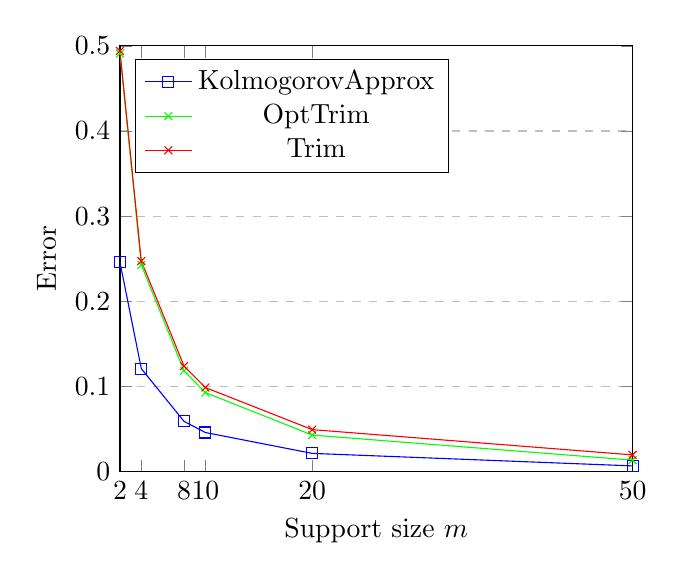
\begin{tikzpicture}
	\begin{axis}[
	scale=.95,
	xlabel={Support size $m$},
	ylabel={Error},
	xmin=2, xmax=50,
	ymin=0, ymax=0.5,
	xtick={2,4,8,10,20,50},
	legend pos=north west,
	ymajorgrids=true,
	grid style=dashed,
	]
	
	\addplot[
	color=blue,
	mark=square,
	]
	coordinates { 
		(2 , 0.246) 
		(4 , 0.121) 
		(8 , 0.0591) 
		(10 , 0.046) 
		(20, 0.0215) 
		(50, 0.0068) 
		
	};
	\addlegendentry{$\KlmApprox$}
	
	\addplot[
	color=green,
	mark=x,
	]
	coordinates {
		(2 , 0.491) 
		(4 , 0.2428) 
		(8 , 0.1184) 
		(10 , 0.0929) 
		(20, 0.0430) 
		(50, 0.0136) 
	};
	\addlegendentry{$\OptTrim$}
	
	\addplot[
	color=red,
	mark=x,
	]
	coordinates {
		(2 , 0.494) 
		(4 , 0.2473) 
		(8 , 0.124) 
		(10 , 0.0988) 
		(20, 0.0494) 
		(50, 0.01971)  
	};
	\addlegendentry{$\Trim$}
	
	\end{axis}
	\end{tikzpicture}
	\caption{Error comparison between $\KlmApprox$, $\OptTrim$, and $\Trim$, on randomly generated random variables as function of $m$.}
	\label{fig:error}
\end{figure}


%\begin{table}[tbp]
%	\scriptsize
%	\centering
%	\begin{tabular}{|c|c|c|c|}
%		\hline
%		m   & $\OptTrim$	& $\Trim$	& Relative error  \\ \hline
%		50  & 0.0193			& 0.0199	& 3.4\%            \\ \hline
%		100 & 0.0093			& 0.0099	& 7.1\%            \\ \hline
%		200 & 0.0043			& 0.0049	& 15.7\%           \\ \hline
%	\end{tabular}
%	\caption{$\OptTrim$ vs. $\Trim$ on randomly generated random variables with original support size $M=1000$.}
%	\label{tab:trimvsoptrim2}
%\end{table}

The above experiments display the quality of approximation provided by the $\KlmApprox$ algorithm, as proven before to be optimal approximation under the Kolmogorv metric. One may wonder the need of such an algorithm where the use of linear programing in an easy valid option described and discussed in previews works~\cite{pavlikov2016cvar}. In order to address this issue we executed an experiment to compare the run-time between $\KlmApprox$ algorithm and a simple linear programing algorithm. The LP algorithm implemented in Mathematics as \hl{follows:...}. The run-time comparison results were very clear and persuasive, for a random variable with support size $n=10$ and $m=5$, the LP algorithm run-time was 850 sec, where the $\KlmApprox$ algorithm run-time was $\approx$ 0 sec. Furthermore, for a random variable with support size $n=100$ and $m=5$, the $\KlmApprox$ algorithm run-time was 0.14 sec and the LP algorithm took significantly much longer, therefore, due to time limitations of the LP algorithm we did not proceed to examine it any farther.
Since it is not trivial to deduce LP algorithm run-time we concluded by the conducted experiment that in this case the LP algorithm might not be as efficient as $\KlmApprox$ algorithm were its run-time is proven to be polynomial~\ref{the:complexity}.


%but it comes with a price tag in the form of run-time performance. The time complexity of both the $\Trim$ operator and the sampling method is linear in the number of variables, resulting in much faster run-time performances than $\KlmApprox$, for which the time complexity is only polynomial (Theorem~\ref{the:complexity}), not linear. The run-time of the exact computation, however,  may grow exponentially. Therefore, we examine in the next experiment the problem sizes in which it becomes beneficial in terms of run-time to use the proposed approximation.


\bibliography{library,Trim_Optimum}{}
\bibliographystyle{abbrv}

\end{document}

